\chapter{Approach and Implementation}
\label{ch:approach

In this chapter the basic work flow is described in detail. The process is mainly drive by an exploratory approach, but follows primarily Farines and Whiteheads~\cite{farine2015constructing} primary steps and key considerations for social network analysis to non-human animal data. The adapted and resulting process is visualized in figure~\ref{fig:process}.

The dataset was first analysed regarding data quality and to form an understanding of the dataset and behaviour of bees in general. Those findings were used to define nodes and infer associations/edges to build the network, respectively derive parameters for the network-generating-pipeline. The static and temporal networks are analysed using network scienc tools and methods (e.g. XXX). For testing hypothesis the networks are combined with attributed data (positions and age information). Each step is explained within the following sections.

\begin{figure}[htb]
	\centering
	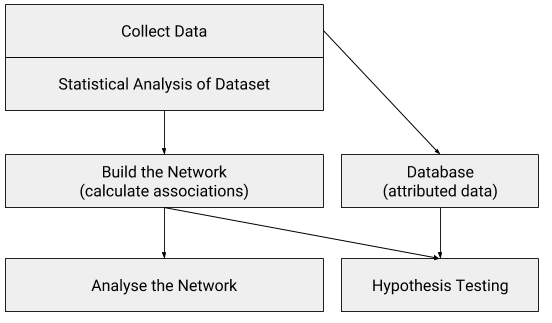
\includegraphics[width=1.0\textwidth]{Figures/WorkProcess}
	\caption{TODO some caption}
	\label{fig:process}
\end{figure}


\section{The Dataset}


\section{Inferring Networks}

\subsection{Network Pipeline}
\subsection{Thresholding Edges}
\subsection{Runtime and Complexity}

\section{Static and Temporal Analysis}	






